\documentclass{beamer}
\beamertemplatenavigationsymbolsempty
\usecolortheme{beaver}
\setbeamertemplate{blocks}[rounded=true, shadow=true]
\setbeamertemplate{footline}[page number]
%
\usepackage[utf8]{inputenc}
\usepackage[english,russian]{babel}
\usepackage{amssymb,amsfonts,amsmath,mathtext}
\usepackage{subfig}
\usepackage[all]{xy} % xy package for diagrams
\usepackage{array}
\usepackage{multicol}% many columns in slide
\usepackage{hyperref}% urls
\usepackage{hhline}%tables
\usepackage{natbib}
\usepackage{natbib}
\usepackage{doi}
\usepackage{mathtools}
% Your figures are here:
\graphicspath{ {fig/} {../fig/} }

%----------------------------------------------------------------------------------------------------------
\title[\hbox to 56mm{Декодирование мозговых сигналов}]{Выбор предсказательной модели в режиме многозадачного обучения с применением методов символьной регрессии}
\author[М.\,Ф. Набиев]{
    Набиев Мухаммадшариф Фуркатович \\
    Научный руководитель: к.ф.-м.н. О.\,Ю.~Бахтеев
}
\institute[Московский физико-технический институт]{
\small{
    Московский физико-технический институт \\
    Кафедра интеллектуальных систем ФПМИ МФТИ 
}}
\date{2024}
%----------------------------------------------------------------------------------------------------------
\begin{document}
%----------------------------------------------------------------------------------------------------------
\begin{frame}
\thispagestyle{empty}
\maketitle
\end{frame}
%-----------------------------------------------------------------------------------------------------
\begin{frame}{Цель исследования}
\textbf{Проблема:} Построение архитектур моделей сильно зависит от априорного знания человека о природе данных, т.е. от их индуктивного смещения. Зная это выбирается соответствующий метод решения. Определение индуктивного смещения автоматическим образом является открытой проблемой.
\newline 
\newline 
\textbf{Цель:} Предложить метод автоматического извлечения индуктивного смещения.
\newline
\newline
\textbf{Решение:} Построение модели, решающей данную задачу, с помощью генетической символьной регрессии и извлечение индуктивного смещения из этой модели.
\end{frame}
%-----------------------------------------------------------------------------------------------------
\begin{frame}{Архитектура решения}
\begin{figure}[t]
        \centering
        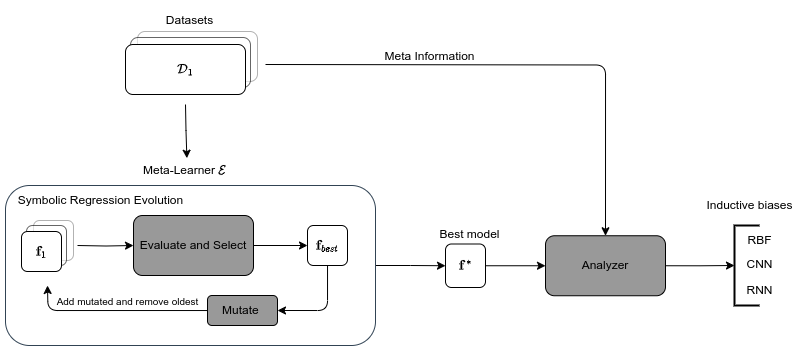
\includegraphics[width=1\textwidth]{model.png}
\end{figure}
Мета-алгоритм \(\mathcal{E}\) принимает на вход наборы данных и эволюционным путем строит модель. Далее лучший кандидат анализируется и делается вывод об индуктивном смещении.
\end{frame}
%----------------------------------------------------------------------------------------------------------
\begin{frame}{Постановка задачи}
Пусть \(\mathfrak{T} = \{T_i\}_{i=1}^n\)~-- множество задач классификации. Каждой задаче \(T_i\) соовтветствует набор данных \( \mathfrak{D}_i = \{(\mathbf{x}_j, \mathbf{y}_j) \}_{j=1}^{N_i} \). Также обозначим \(\mathfrak{S} = \{ \mathfrak{D}_i\}_{i=1}^n\) и \(\mathfrak{F}\)~-- множество всех моделей.
\begin{itemize}
    \item Модель \(\mathbf{f} \in \mathfrak{F}\) определяется набором из трех функций \texttt{Setup}, \texttt{Learn}, \texttt{Predict}.
    \item Мета-алгоритм \(\mathcal{E}: \mathfrak{S} \rightarrow \mathfrak{F}\) представляет из себя генетический алгоритм, который конструирует модель путем символьной регреcсии. 
    \item Пусть \(
        \operatorname{mACC}(\mathbf{f}, \mathfrak{S}) = \frac{1}{n} \sum_{i=1}^{n} \sum_{j=1}^{N_i} \frac{[f(\mathbf{x}_j) = \mathbf{y}_j]}{N_i}
    \). Тогда задача оптимизации сводится к нахождению наилучшей модели
    \[
        \mathbf{f}^* = \arg \max_{\mathbf{f} \in \mathfrak{F}} \operatorname{mACC}(\mathbf{f}, \mathfrak{S}_{\text{test}}).
    \]
\end{itemize}

\end{frame}
%----------------------------------------------------------------------------------------------------------
\begin{frame}{Данные для эксперимента}
Для экспериментов использовались выборки \texttt{cricles} из \texttt{sklearn}. Выборки отличаются расположением центра концентрических кругов.

\begin{columns}[c]
\column{0.5\textwidth}
\begin{figure}
    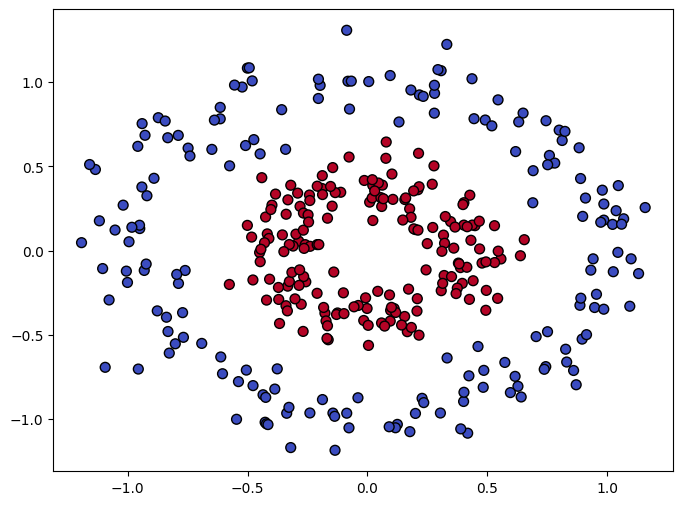
\includegraphics[width=0.9\textwidth]{circles.png}
    \caption{Пример одной выборки.}
\end{figure}
\column{0.5\textwidth}
\begin{itemize}
    \item Количество выборок было равно 10. В каждом из них было по 100 элементов.
    \item Максимальная длина функций \texttt{Learn} и \texttt{Predict} была взята равной 10.
\end{itemize}
\end{columns}
\textbf{Гипотеза:} код модели будет содержать элементы вычисления радиально-базисного ядра или схожих функций.
\end{frame}
%----------------------------------------------------------------------------------------------------------
\begin{frame}{Результаты эксперимента}
\begin{columns}[c]
\column{0.5\textwidth}
\begin{figure}
    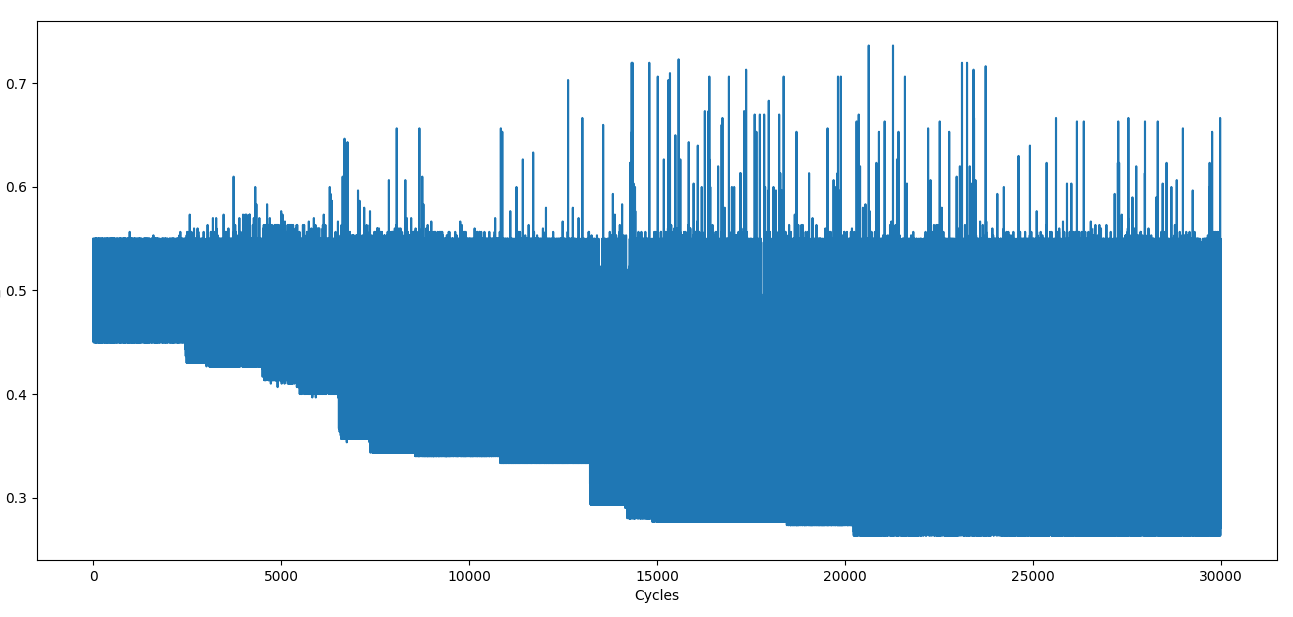
\includegraphics[width=1\textwidth]{acc_loss_mid.png}
    \caption{График \(1 - \text{accuracy}\).}
\end{figure}
\column{0.5\textwidth}
\begin{figure}
    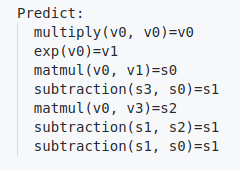
\includegraphics[width=0.7\textwidth]{predict.png}
    \caption{Функция \texttt{Predict} лучшей модели.}
\end{figure}
\end{columns}
Формальная запись функции имеет вид
\[
    s_3 - 2(\mathbf{x} \odot \mathbf{x})^{\intercal}e^{\mathbf{x} \odot \mathbf{x}} - (\mathbf{x} \odot \mathbf{x})^{\intercal} \mathbf{v}_3,
\]
где \(\mathbf{v}_3\) и \(s_3\)~-- веса модели. Данное представление близко к радиальным базисным функциям, которые являются индуктивным смещением данных.
\end{frame}
%----------------------------------------------------------------------------------------------------------
\begin{frame}{Дальнейшие исследования}
\begin{itemize}
    \item Добавить анализатор для извлечения индуктивного смещения из модели.
    \item Добавление регуляризации учитывающей вложенность функций.
    \item Проведение экспериментов на выборках с индуктивным смещением CNN и RNN.
    \item Результаты будут доложены на конференции МФТИ.
\end{itemize}
\end{frame}
%----------------------------------------------------------------------------------------------------------
% \begin{frame}{Источники}
%     \bibliographystyle{plain}
%     \bibliography{ib_in_model_selection}
% \end{frame}
%-----------------------------------------------------------------------------------------------------


\end{document} 
